\section{Zajęcia dydaktyczne}
\subsection{Wejściówka}

Na samym początku zajęć odbędzie się wejściówka składająca się z pytań otwartych
i zamkniętych.
Przykładowe pytania które mogą znaleźć się na wejściówce to:

\begin{enumerate}
    \item Podaj definicję dodawania i mnożenia w $\mathbb{F}_2$ bądź wypisz wynik tych
    działań dla wszystkich możliwych kombinacji elementów.
    \begin{itemize}
        \item Odpowiedź: Tablica~\ref{truth_table:title} bądź~(\ref{modulo_addition})
        oraz~(\ref{modulo_multiplication})
    \end{itemize}
    \item Ile błędnych symboli jest w stanie wykryć oraz poprawić kod Reeda-Solomona
    \begin{enumerate}[label=\Alph*:]
        \item wykryć: $n-k$, poprawić: $n-k-1$
        \item wykryć: $n-k-1$, poprawić: $n-k-1$
        \item wykryć: $\lfloor \frac{n-k}{2} \rfloor$, poprawić: $\lfloor \frac{n-k}{2} \rfloor$
        \item wykryć: $n-k$, poprawić: $\lfloor \frac{n-k}{2} \rfloor$
    \end{enumerate}
    \item Podaj zaletę oraz wadę stosowania większej ilości poziomów w modulacjach PAM
    \begin{itemize}
        \item Zaleta: jeden symbol koduje więcej bitów - więcej bitów jest przesyłanych w jednym cyklu zegara
        \item Wada: różnica między poszczególnymi symbolami maleje, a więc trudniej jest rozróżnić symbole
    \end{itemize}
    \item Czym się różni szerokość pasma od przepustowości?
    \item Opisz krótko czym jest NRZ (Non-Return-to-Zero)
    \item Czym jest przepływność łącza?
    \item Która biblioteka wykorzystywana jest do stworzenia GUI?
    \begin{enumerate}[label=\Alph*:]
        \item Tkinter
        \item PyQt --- Odpowiedź prawidłowa w punkcie~\ref{subsection:interfejs}
        \item OpenGL
        \item WindowsForms
    \end{enumerate}
\end{enumerate}

\subsection{Narzędzia}

W trakcie zajęć laboratoryjnych student będzie miał do dyspozycji symulator phyether, który zawiera implementację wybranych rozwiązań
części standardów 25GBASE-T i 40GBASE-T.

\subsection{Ćwiczenie dydaktyczne --- modulacje PAM}

\subsubsection{Wstęp teoretyczny}

Modulacja cyfrowa to technika zamiany bitów na sygnał oraz sygnału na bity. Jest kluczowym zagadnieniem w przesyle danych pomiędzy systemami
komputerowymi. Technologie Ethernetowe wykorzystują wiele technik modulacji. Ćwiczenie te ma na celu przybliżenie oraz porównanie
występujących technik modulacji PAM (Pulse-Amplitude Modulation), która jest jedną z najpopularniejszych w technologii Ethernet.

Najprostszym schematem modulacji jest NRZ --- Non-Return-to-Zero. Chcąc przesłać bit o wartości $0$, na skrętkę zostanie podany sygnał
ujemny, a w przypadku $1$ --- dodatni. Rozwiązanie te niesie za sobą parę wad. Przykładowo, gdy nadawane są długie ciągi zer lub jedynek, sygnał
nie ulega zmianie --- jest to zjawisko niepożądane podczas transmisji i może doprowadzić do desynchronizacji zegarów strony nadawczej i odbiorczej.
Z uwagi na to, NRZ wykorzystywany jest w praktyce w połączeniu z np. kodowaniem liniowym 64b/66b w celu uniknięcia sekwencji zer i jedynek.

PAM jest modulacją, w której dane przesyłane są w postaci zmian amplitudy sygnału. Zmiany te nazywane symbolami. Modulacje PAM różnią się między sobą
liczbą wykorzystywanych poziomów modulacji. PAM3 wykorzystuje trzy poziomy, PAM4 --- cztery, PAM16 --- szesnaście. NRZ można wobec tego nazwać PAM2.
Powodem dla którego zwiększenie poziomów ma sens jest zwiększona szybkość transmisji. Weźmy na przykład PAM4 --- mając cztery poziomy mamy
do dyspozycji cztery symbole $-3$, $-1$, $1$, $3$, a więc każdy symbol kodować może dwa bity danych. W przypadku NRZ, jeden symbol koduje tylko jeden bit.
Zatem zwiększenie liczby poziomów pozwala na przesył większej ilości bitów przy użyciu jednego symbolu. Schemat ten będzie działa o ile strona odbiorcza
potrafi rozróżnić poszczególne symbole od siebie, jest to jednak łatwiej osiągalne niż zwiększenie szerokości pasma.
Modulacje PAM4, PAM16 i inne, analogicznie jak NRZ, podatne są na długie ciągi zer i jedynek. Dlatego niezbęde jest zastosowanie różnych "gmatwaczy" bitów, które
zamienią takie sekwencje na bardziej zróżnicowany ciąg np. skrambler.

\subsubsection{Opis narzędzia}

Program phyether, w zakładce "PAM", posiada symulator modulacji NRZ, PAM4 oraz PAM16, który ilustruje zachowanie sygnału w skrętce podczas transmisji, w zależności
od wybranych modulacji.
Narzędzie będzie wykorzystywane podczas tej części ćwiczenia.

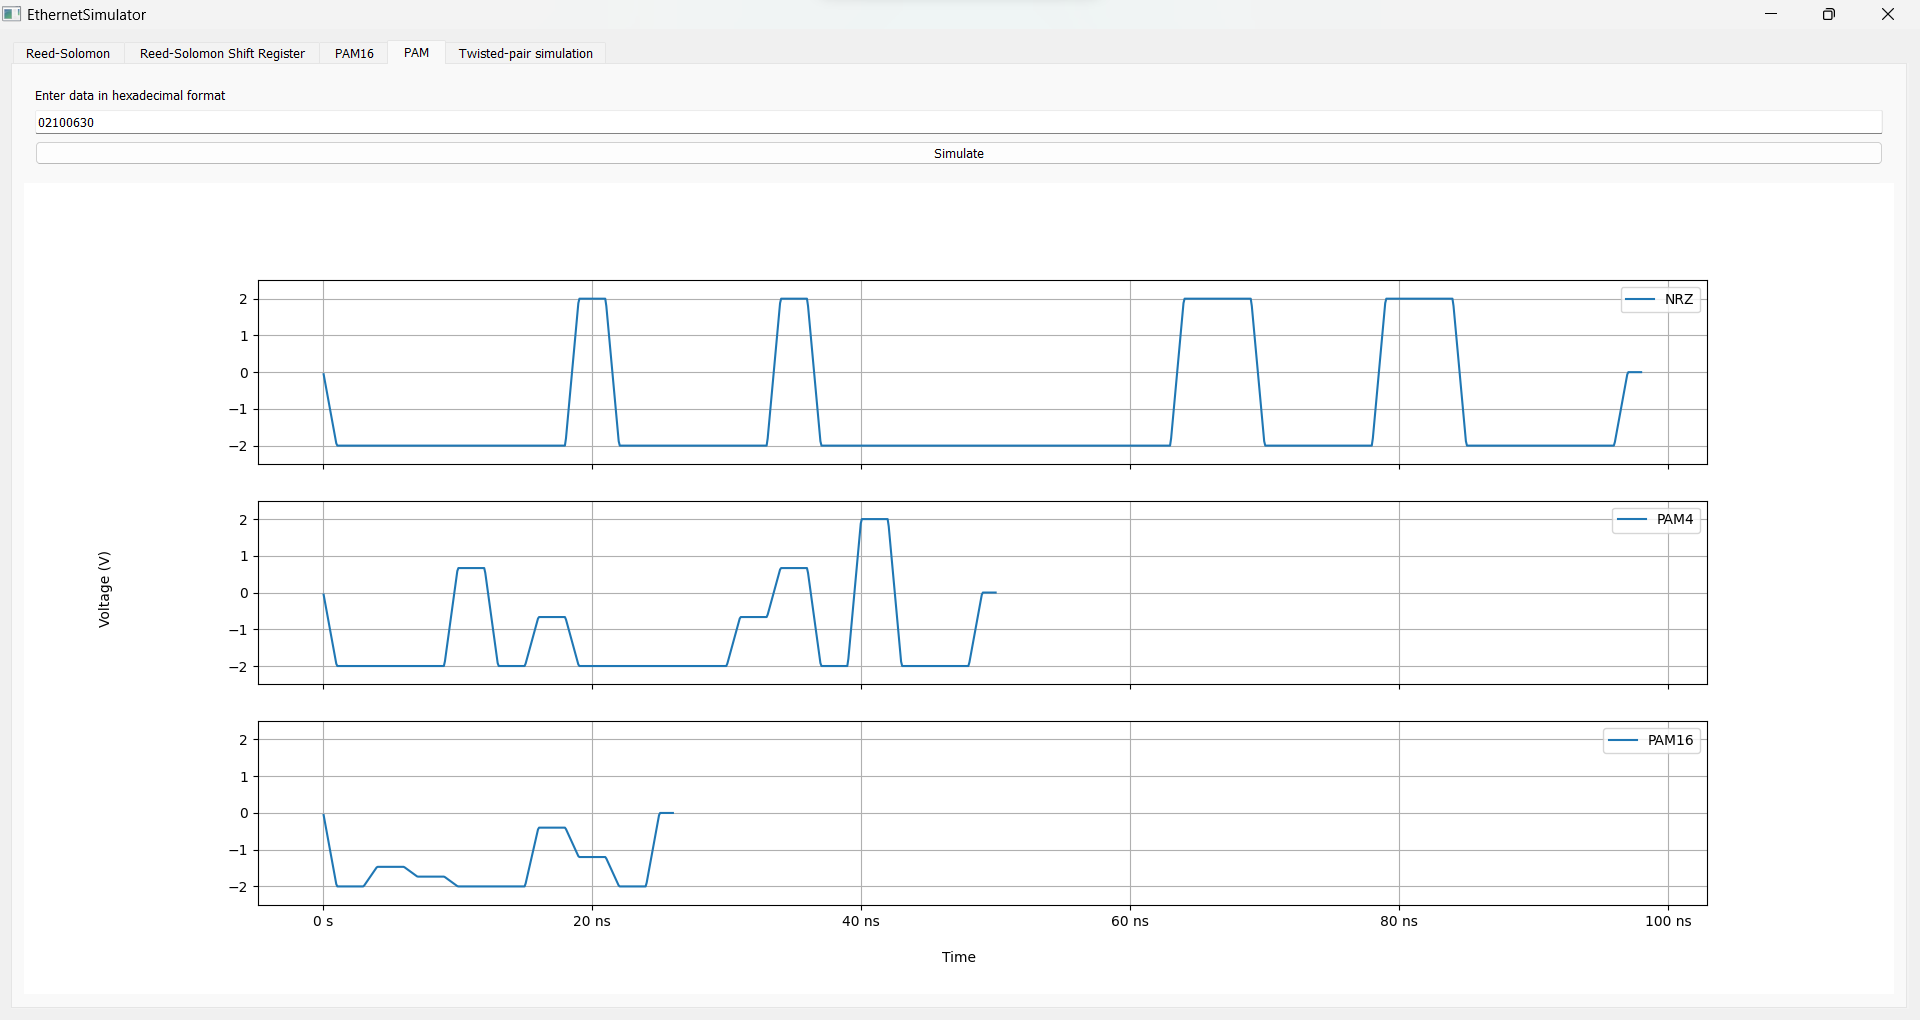
\includegraphics[scale=0.37]{pam_tab.png}

Powyższa grafika prezentuje zakładkę "PAM" programu phyether. Nad przyciskiem \textbf{Simulate} znajduje się pole tekstowe, do którego wpisane mogą być dane w formie
liczb w systemie szesnastkowym. Po wpisaniu danych i kliknięciu \textbf{Simulate}, wpisane dane zamieniane są na symbole modulacji NRZ, PAM4 oraz PAM16, które
następnie wysyłane są na medium. Wynik symulacji przedstawiony jest w dolnej części zakładki.

\subsubsection{Zadania do realizacji}

\begin{enumerate}
    \item Zamień numer swojego indeksu na postać szesnastkową i wykorzystaj go jako liczbę do przesłania. Przeprowadź symulację. Zanotuj w sprawozdaniu
    przybliżony czas transmisji oraz liczbę poziomów natężenia. Opisz wnioski, które nasuwają Ci się po wykonanym ćwiczeniu.
    \item Prześlij ciąg składający się z samych jedynek (fffffff \dots). Popatrz na wynik symulacji. Jak nazywa się zaobserwowane zjawisko? Czy znasz sposoby,
    które zapobiegają jego wystąpieniu? Zanotuj w sprawozdaniu.
\end{enumerate}
